\newpage
\sect{3 \quad Our challenge, philosophy and hypothesis}
\textbf{Assumption and failure case.} IDEC uses reconstruction to keep the embedding informative. The details that reduce pixel error can include information irrelevant to a chosen clustering task [1,4]. Consider a handwritten 7 with a small cross in the margin. Remembering where the cross sits helps a decoder draw it. Moving it has no bearing on which digit was written. A model could encode that information and still cluster digits correctly, so we measure both what its decoder reproduces and what changes its final assignments.

\textbf{Our philosophy.} Define relevance relative to the intended grouping. For digit identity, the same handwriting should retain its cluster across a change in decoration. Two aligned views of the same digit let us identify pixels that persist under a controlled change. This supplies a training target for reconstruction without using a digit label. A Gaussian prior assumes that central pixels tend to be more informative because MNIST digits are usually centered.

\textbf{Prior evidence and prediction.} Our earlier stripe experiment changed pixel values over the entire image, including the strokes. Under strong stripes, projecting a known contrast out of the pretraining loss reduced final flips from 39.53\% to 2.61\% with projected fine-tuning held fixed. That motivated intervening during pretraining. For the present experiment we predicted fewer switches under movement of a detached mark, then tested shape changes and digit accuracy separately (\href{https://github.com/JohnR31N/cs126FinalProj/blob/62b24eb/IDEC/background/design.md}{design before fitting}).

\begin{center}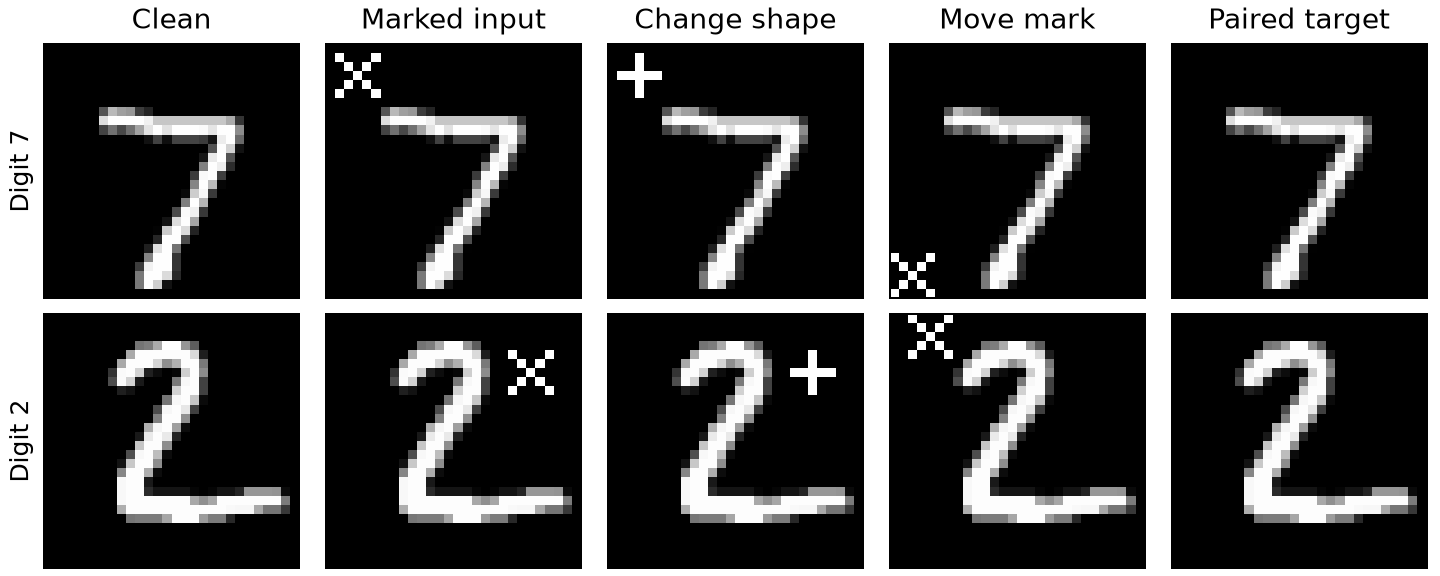
\includegraphics[width=.92\linewidth]{../figures/geometry.png}\end{center}
\smallcap{\textbf{Figure 1.} The first two test digits. Changing shape keeps the site fixed. Moving the mark keeps its shape fixed. The final column is computed from the marked input and moved view. Every ink pixel, including faint edges, retains its original value.}

\sect{4 \quad Proposed modification and controls}
\textbf{Paired reconstruction target.} Let $u$ and $v$ contain the same digit with a mark at disjoint sites. For pixel $j$, set $t_j=u_j$ if $u_j=v_j$, and $t_j=0$ otherwise. A decoder trained on an augmented view minimizes its MSE to $t$. This is a denoising objective [6]. The controlled pair supplies the target. Under this construction $t$ exactly recovers the digit on black, as we verified on every image. The network receives one image at inference.

\textbf{Competing explanations.} Standard pretraining reconstructs one fixed marked image per digit. Augmentation alone resamples the shape and site each epoch and reconstructs the current view. Paired-target training uses the same augmented inputs with target $t$. The fourth arm uses those inputs with the full target, but weights each squared pixel error by $w_j\propto\exp[-\|j-(13.5,13.5)\|^2/(2\cdot7^2)]$, normalized to mean one. This fixed Gaussian supplies a location preference without learning attention weights.

\newpage
\sect{5 \quad Experimental setup}
We used the same 12,000 training and 10,000 held-out MNIST digits across all four arms. A plus and a diagonal cross each occupy nine white pixels in a $5\times5$ box. For each digit we chose two disjoint boxes with at least one blank pixel of clearance from every nonzero stroke pixel. Location depends on available blank space. Shape assignment was balanced and randomized independently of digit labels. The three augmented arms sample the same sequence of four shape/site combinations for each seed. Only paired-target training uses the alignment between views to build its target.

For each seed (0--4) all arms used the same random initial weights and minibatch order, 100 pretraining epochs and the architecture in our code ($784,500,500,2000,10$ encoder, mirrored decoder). K-means with 20 restarts initialized ten centers for each resulting embedding. All arms then ran ordinary full-image IDEC on the fixed marked training views for 5,600 Adam updates (learning rate $10^{-3}$, batch size 256, target refresh every 140 updates).

\textbf{Readouts.} We learn cluster names from training labels after optimization and freeze that mapping. Each model sees the same test digits clean, marked, with the shape swapped, and with the mark moved. The primary measure is the fraction of cluster IDs that change when the mark moves. Clean and marked accuracy use the same frozen model. We also record accuracy for the quarter of test digits whose ink centroids lie farthest from the image center.

An exploratory decoder check replays pretraining and compares two reconstructions of the same digit with the mark at two sites. For decoder outputs $\hat u,\hat v$ the score is $(\hat u-\hat v)^\top(u-v)/\|u-v\|^2$. A score of one reproduces the full signed change along the displacement. Zero indicates no response along that direction. This reads information used by the decoder; other information may remain in the embedding.

\sect{6 \quad Results and analysis}
\begin{center}\small
\setlength{\tabcolsep}{3pt}
\begin{tabular}{lrrrrr}
\toprule
Pretraining & Marked ACC & Clean ACC & Move flips & Shape flips & Decoder response\\
\midrule
Full, fixed input & 67.15 & 69.84 & 6.20 & 5.35 & 0.00585\\
Augmentation only & 71.02 & 72.96 & 4.34 & 3.43 & 0.00313\\
Aug. + paired target & 71.55 & 73.02 & 4.18 & 3.59 & 0.00085\\
Aug. + Gaussian & 72.91 & 74.34 & 4.16 & 3.37 & 0.00278\\
\bottomrule
\end{tabular}

\end{center}
\smallcap{\textbf{Table 2.} Five-seed means. Accuracy and flip rates are percentages. The decoder response is dimensionless and is measured just after pretraining. The other four columns evaluate final clusters. All individual runs and paired differences are included with the report.}
Moving the mark changed 6.20\% of assignments under ordinary IDEC. Augmentation reduced this to 4.34\%, a paired reduction of $1.86\pm0.52$ percentage points (mean $\pm$ seed SD). Swapping the shape at the same site produced a similar reduction, from 5.35\% to 3.43\%. Both rates fell for every seed. The same fixed-input models achieved 69.84\% accuracy on clean images and 67.15\% on marked versions of those digits. Preserving the original ink therefore still left a measurable effect of the test-time decoration.

With augmentation held fixed, the paired target further reduced movement flips by $0.15\pm0.24$ points but \emph{increased} shape flips by $0.16\pm0.18$ points. Its extra gain in marked ACC was $0.53\pm6.45$ points. The Gaussian prior gave the highest mean marked ACC, a paired $1.88\pm2.69$ points above augmentation alone. Its additional reduction in movement flips was $0.18\pm0.31$ points. The small differences among the augmented arms and their variability limit any ranking of their stability.

The baseline decoder weakly tracked the mark's displacement (0.00585 on a scale where one means full tracking). Augmentation reduced the response to 0.00313. The paired target lowered it further to 0.00085 in the five-seed mean, with a reduction in every seed. This change in reconstruction had a much smaller and less consistent effect on final cluster assignments.


\newpage
\sect{7 \quad Limitations and conclusion}
\textbf{Choice of method.} Background augmentation accounted for most of the observed reduction in movement flips. A paired reconstruction target directly implements our hypothesis about relevance. It needs aligned views that retain the handwriting while changing the decoration. The Gaussian needs only a center and a width. Across the test set its mean normalized pixel weight was 1.79 on ink and 0.67 on the mark. Even in the outermost quartile of digit centroids, its mean marked ACC was 73.11\% compared with 71.14\% under augmentation alone. The farthest MNIST test centroid was only 1.41 pixels from the image center. This subgroup cannot establish robustness to substantially displaced digits.

\textbf{Limits of the relevance assumption.} In this construction all stroke pixels stay fixed and the two mark sites are disjoint, so equality across the paired views yields a clean target. Repeated background features could also be stable, and pose changes could move relevant foreground pixels. A fixed Gaussian can downweight an off-center stroke or upweight a central distractor. Site selection here avoids the handwriting, so where a mark can appear depends on the available blank space. The findings cover this family of decorations, this split and five seeds. A separate test with displaced digits and backgrounds near the image center would probe the limits of the spatial prior.

\textbf{Relation to the earlier experiments.} The \href{https://github.com/JohnR31N/cs126FinalProj/blob/idec-final-v1.4/IDEC/report/report.pdf}{additive-overlay study} tested a known, fixed stripe direction and crossed reconstruction losses across the two training stages. Those stripes changed intensities on the digit as well as in the surrounding space. Here the foreground pixels stay exactly fixed, and the paired target is constructed without the shape masks or a known stripe direction. Each study has its own matched baseline. The difference in their numerical effect sizes also reflects the extent, strength and type of intervention.

